\documentclass[]{article}
\usepackage{amssymb}
\usepackage{amsfonts}
\usepackage{amsmath}
\usepackage{graphicx}
\usepackage{float}


\restylefloat{table}
\title{Trabajo Practico N\'umero 1: Grupo EconoDatos}
\author{Mart\'n Yanquilevich, Federico Paci, Leonardo Esteban Delgado, Mart\'in Gerschenfeld}
%opening

\begin{document}
\maketitle
\tableofcontents
\newpage




\section{Introducci\'on}

Link del Repositorio: https://github.com/Martingerschenfeld/Tp-Datos/\\

El trabajo pr\'actico 1 de la materia se basa en el an\'alisis de los tweets del set de datos de Kaggle. El objetivo es hacer un an\'lisis exploratorio sobre los datos que surgen de twitter, relacionado con eventos del tipo desastres naturales. \\

El set de datos contiene 10,000 tweets seleccionados a mano por la pagina Kaggle. Los tweets se encuentran relacionados con palabras claves de desastres naturales. En muchos casos, usuarios utilizaron palabras metaf\'oricas para referirse a otras situaciones, pero ajeno a desastres naturales. Tal como podemos ver en el siguiente ejemplo, donde la usuaria "Anna K" se refiere al cielo naranja como si se estuviera incendiando. Este tipo de tweet puede ser captado por el data-set. El objetivo del dato es extraer estad\'isticas y llegar a conclusiones sobre la posibilidad de determinar si Twitter es un lugar confiable para informarse acerca de cat\'astrofes naturales.

\begin{figure}[H]
	\centering
	
\includegraphics[width=0.75\linewidth]{tweet_screenshot}
	\caption[]{Tweet extraido de Kaggle.com}
\end{figure}

\section{An\'alisis Exploratorio de Datos}

Arrancamos el ejercicio cargando los datos como un Pandas Dataframe desde el csv de la pagina de Kaggle. \\

El dataframe consiste en 5 columnas:
\begin{itemize}

\item id - identificador \'unico para cada tweet
\item text - el texto del tweet
\item location - ubicación desde donde fue enviado (podr\'ia no estar)
\item keyword - un keyword para el tweet  (podr\'ia no estar)
\item target - en train.csv, indica si se trata de un desastre real  (1) o no (0)
\end{itemize}
 
 Haciendo un info sobre el DataFrame podemos observar que contiene 5 columnas y 7613 filas no nulas. Las columnas id es un numero (integer con longitudad m\'axima de 64 caracteres) , as\'i como el target (que adem\'as es binario, vale o bien 0 o 1), por lo que tiene sentido. Las otras tres columnas, corresponden a textos, en Python esto se representa como un string, que es un tipo "object" (que es  el formato en Python de todo lo que no es un integer, boolean, ect.). Vemos que las Pandas logr\'o identificar correctamente que tipo de datos son en cada columna. \\
 De las filas, algunas columnas tienen componentes nulos. El id (que funciona como key) y el texto del tweet son los \'unicos completos. En algunos tweets, no est\'a establecido la ubicaci\'on, en otros casos no fue identificado la keyword que mejor identifica el contenido del tweet, ni tampoco si el tweet es veraz o no (target puede ser NaN). 
 
 \begin{figure}[H]
 	\centering
 	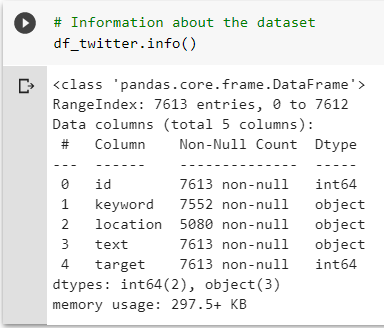
\includegraphics[width=0.75\linewidth]{df_twitter.info}
 	\caption[]{Info de los Tweets extra\'ido de Kaggle.com}
 \end{figure}
\section{Palabras m\'as utilizadas}
Resulta interesante ver cuales son las palabras m\'as utilizadas para identificar la utilidad de twitter en situaciones de cat\'astrofes naturales.\\

El primer paso consisti\'o en transformar los textos de los tweets en una lista (de la misma dimensi\'on que id). Luego buscamos separar palabra por palabra para obtener una lista con el mismo tamaño a la cantidad de palabras de todos los tweets (113 461). Como paso intermedio a contar palabras, primero convertimos todas las palabras a min\'uscula. Python es case-sensitive a la hora de realizar operaciones, por lo que dos palabras iguales, donde la primera letra es may\'uscula es considerada como una palabra distinta. Finalmente, realizamos un for que toma un diccionario vac\'io, luego se fija cada palabra en la lista, en caso de no encontrarla en el diccionario, entonces la agrega con un conteo de 1, en caso de que ya exista un registro, entonces le suma el conteo por 1. Finalmente, se ordena el diccionario de mayor value a menor. \\

Observando el resultado de los 15 resultados m\'as frecuentes vemos que no resulta informativo. Las palabras m\'as utilizadas son art\'iculos, pronombres, ect. Resulta m\'as \'util si estas palabras fueran sustantivos o tal vez adjetivos, por lo que debemos volver a filtrar. \\  

 \begin{figure}[H]
	\centering
	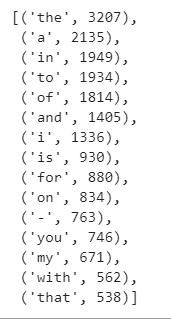
\includegraphics[width=0.35\linewidth]{tweet_token}
	\caption[]{Las 15 palabras m\'as frecuentes en los tweets del data set}
\end{figure}

Para obtener mejor informaci\'on sobre las palabras m\'as frecuentes, observamos que las 15 palabras m\'as frecuentes ten\'ian 4 letras o menos. Por ende el filtro que aplicamos fue tomar las palabras que ten\'ian por lo menos 5 letras. Este filtro no es el m\'as preciso y existe el riesgo de que vayamos a eliminar palabras de 3 o 4 letras relevantes, sin embargo consideramos que es efectivo para poder tener informaci\'on r\'apida. \\

En el siguiente histograma presentamos las 15 palabras m\'as frecuentes de por lo menos 5 letras y su frecuencia. 
 \begin{figure}[H]
	\centering
	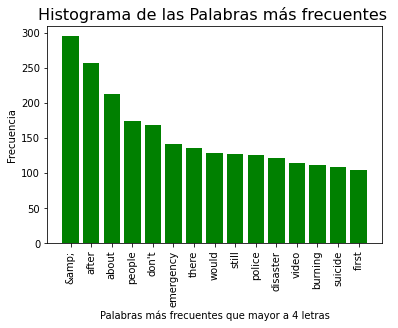
\includegraphics[width=0.75\linewidth]{histograma1}
	\caption[]{Las 15 palabras de m\'as de 4 letras m\'as frecuentes en los tweets del data set}
\end{figure}

Si bien no podemos identificar si los tweets son relacionados con cat\'astrofes naturales, y habr\'ia que verlas en su contexto, las palabras que figuran en el histograma son, por lo menos pertinentes. Para ejemplificar, observamos las palabras desastre, emergencia y quemando, que son descripciones del hecho. Encontramos las palabras personas y polic\'ia, que son sujetos intervinientes, y encontramos palabras como suicidio, y despu\'es que hablan de las consecuencias de la cat\'astrofe. Como hecho negativo del filtro, encontramos en el listado tambi\'en la palabra \&amp, que luego de buscar el significa en internet, resulta que es parte de un codigo de html, por ende fue un error en el cargado de los tweets al csv. 

\section{An\'alisis por ubicaci\'on}

La columna 'location' del DataFrame contiene informaci\'on sobre el lugar donde se env\'io el tweet. Resulta interesante analizar, puesto que si tuvi\'eramos informaci\'on acerca de cat\'astrofes naturales que ocurrieron, entonces se podr\'ia comparar, y ver con mayor detalle la importancia de twitter. La informaci\'on de ubicaci\'on es auto-reportada y no est\'a sujeto a verificaci\'on. \\

Un an\'alisis preliminar muestra la siguiente informaci\'on.\\
 \begin{figure}[H]
	\centering
	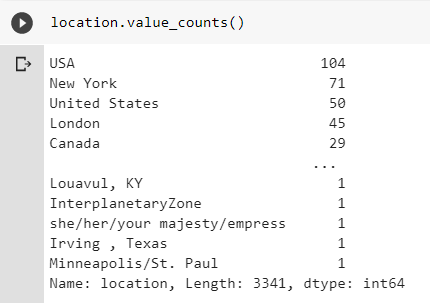
\includegraphics[width=0.75\linewidth]{location}
	\caption[]{Ubicaci\'on auto reportada del data set}
\end{figure}

Observamos que Twitter no agrupa dicha informaci\'on en pa\'ises, sino que copia textualmente el valor. Ocurre que hay ubicaciones que se encuentran abreviadas (Por ejemplo USA, representa el mismo pa\'is que United States of America), hay personas que han puesto su estado o ciudad (New York o California son dos estados dentro de Estados Unidos), hay personas que han escrito mal su ubicaci\'on, hay personas que escribieron el nombre su pa\'is en su idioma natal y cuesta comparar con el nombre en ingles (Brasil en vez de Brazil), espacios en el nombre de los pa\'ises que lo hace imposible distinguir para Twitter y una gran cantidad de personas pusieron de ubicaci\'on lugares inexistances o frases sin sentido (tal como she/her/your magesty/empress). \\
Para conseguir mejores resultados en este apartado, hicimos reemplazos para homogeneizar los nombres al idioma ingles. Por un tema de tiempo y eficiencia, fue hecha para todos los valores cuya frecuencia fue mayor a 3. No hemos encontrado una regla sistem\'atica, y si bien se puede seguir haciendo cambios, consideramos que no modifica sustancialmente el resultado. \\
Para hacer dicho cambio, armamos una diccionario cuyo key es el string del texto que queremos cambiar y el value es el pa\'is al cual pertenece. En caso de que no fuera identificable, se le aplic\'o el valor nulo de NaN. Luego mapeamos el diccionario a location, completando lo no identificado con NaN. Observamos a continuaci\'on los resultados.

 \begin{figure}[H]
	\centering
	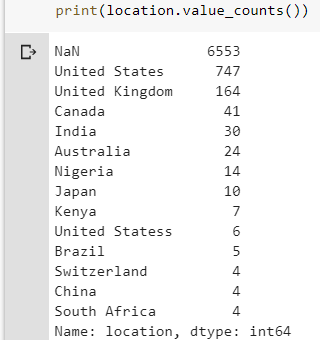
\includegraphics[width=0.75\linewidth]{location2}
	\caption[]{Ubicaci\'on del auto reportada que realiz\'o el tweet - Corregido}
\end{figure}

Observamos cambios notorios con respecto a la tabla anterior. Mientras que en antes los Estados Unidos figuraba como las primeras 3 entradas, ahora lo tenemos condensado en una sola entrada y por ende es m\'as representativo. En este punto, decidimos simplemente observar los gr\'aficos, y considerar el resultado cualitativo debido a la poca confiabilidad de los datos NaN. Para concluir de la tabla 2, podemos decir Estados Unidos es el pa\'is donde la gran mayor\'ia de los tweets provienen de, luego en una menor cuant\'ia sigue el Reino Unido, luego en una menor medida varios pa\'ises, que no podemos garantizar significativamente cual es m\'as frecuente. 

\section{An\'alisis por Longitud del Tweet}
Para el siguiente apartado, analizamos la longitud de los tweets del data set, recordamos que hasta el 2017, los limites de caracteres que se puede tener en un tweet es de 140, luego de dicha fecha el limite fue aumentado a 280. Desconocemos el año del data set, sin embargo es de presumir que es pre 2017. 

 \begin{figure}[H]
	\centering
	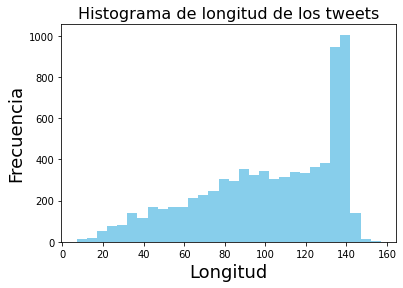
\includegraphics[width=0.75\linewidth]{longitud}
	\caption[]{Histograma de longitud de los Tweets}
\end{figure}

Observamos que la moda son valores cercanos al limite de 140 caracteres. Este resultado tiene sentido, puesto que es esperable que en situaciones extremas, las personas se sientan inclinados por expresar emociones, deseos de recuperación ajena o criticas a gobiernos por no estar suficientemente preparado. Otro punto a tener en cuenta es que existen tweets con longitud mayor a 140, lo m\'as probable es que sean anomal\'ias, o errores en la carga al csv. De todas formas, recomendamos mirar m\'as de cerca los datos para evaluar que hacer con estos datos.\\

Para continuar nuestro an\'alisis de longitud, podemos incorporar el elemento de la veracidad. La variable 'target' es una variable binaria donde si vale 1 entonces el tweet se encuentra relacionado con un hecho real, y si el valor es 0, o bien no se encuentra relacionado, o no se sabe (nuestro supuesto inicial). Repetimos nuestro an\'alisis de longitud de tweets, tomando en cuenta el valor de veracidad. 

 \begin{figure}[H]
	\centering
	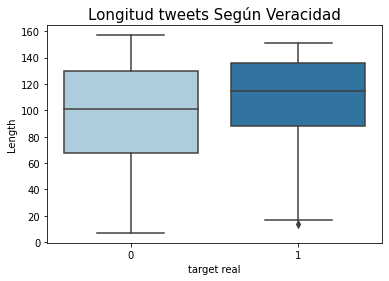
\includegraphics[width=0.75\linewidth]{longitud2}
	\caption[]{Histograma de longitud de los Tweets en funci\'on de la veracidad}
\end{figure}

Utilizamos un gr\'afico de caja y bigote. En celeste, son los tweets con veracidad 0, se observa un rango amplio de 10 a 150, con media en 100 y cuartiles en 70 y 150. En la caja azul, se observa un rango entre 20 y 140 , con media en 110 y cuartiles en 90 y 135. En primer lugar, pareciera que en el caso de la veracidad igual a 1, los tweets son significativamente y consistentemente m\'as alto. Esto se puede ver por el rango m\'as chico, la media y los cuartiles 1 y 3 m\'as altos. No se puede garantizar si esto es as\'i siempre, pero gr\'aficamente se puede apreciar una intuici\'on: Si el tweet es m\'as largo, entonces es m\'as probable que sea relacionado a un evento real que no. 

\section{An\'alisis de los Keywords}
Una de las caracter\'isticas de los tweets del dataset es el keyword, que es una variable categ\'orica, tweets con el mismo keyword se agrupan entre s\'i. De los 7613 tweets originales, 7552 tiene categor\'ias, de las cuales se pueden agrupar en 221 categor\'ias distintas. Si bien, muchos de los tweets no est\'an relacionados con catastrofes naturales, decidimos trabajar con un subset de datos para poder filtrar mejor y llegar a conclusiones m\'as significativas. \\

El primer criterio de filtraci\'on fue quedarnos con las keywords que aparecen m\'as veces que el la aparici\'on promedia de keywords. Eso redujo las 221 categor\'ias a 114. Luego elegimos quedarnos con tengan poro lo menos 39 frecuencias. A continuaci\'on observamos el histograma de las frecuencias. \\

 \begin{figure}[H]

	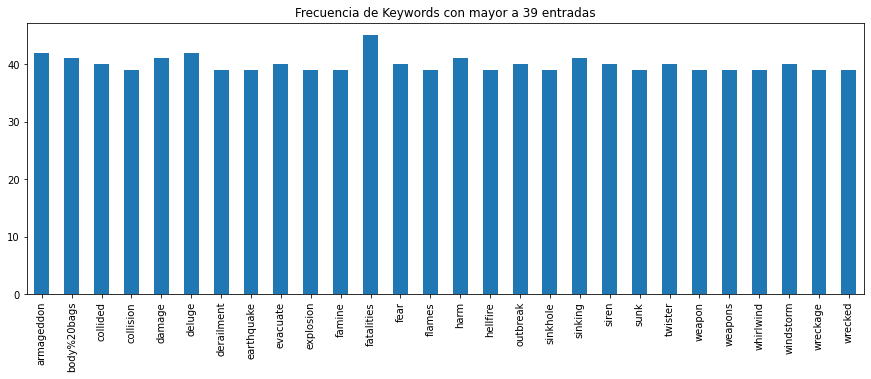
\includegraphics[width=1.20\linewidth]{keyword}
	\caption[]{Frecuencia de 38 keywords m\'as frecuentes}
\end{figure}

Si observamos las keywords de las m\'as frecuentes, observamos que son relevantes con cat\'astrofes naturales, por ejemplo: armageddon, body bags, collision, damage, earthquake, ect. \\


Para seguir con nuestro an\'alisis, analizamos como son las keywords en funci\'on de la veracidad. Para ello, clasificamos la cantidad de veces que aparece cada keyword en el caso de que el tweet tenga target == 0 y target == 1, para luego encontrar el porcentaje veracidad que tiene cada keyword. 

 \begin{figure}[H]
	
	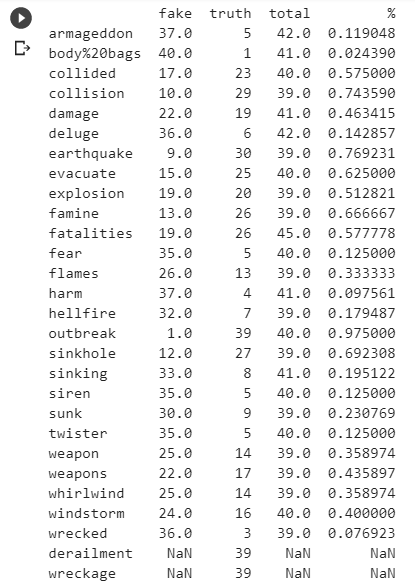
\includegraphics[width=1.20\linewidth]{keyword2}
	\caption[]{Frecuencia y \% de veracidad por keywords}
\end{figure}

Yendo en mayor detalle de la veracidad, podemos ver que categor\'ias que eran muy frecuentes en el gr\'afico anterior, pueden no tener que ver con desastres naturales. Para ejemplificar, el caso de body bags, tiene 41 instancias, de las 40 son falsas y 1 es verdadera. Mientras que categor\'ias como brote (outbreak) tiene 40 instancias, de las cuales 39 fueron relacionados con un hecho real.\\

Gráficamente podemos observar lo expresado en la tabla.  \\

 \begin{figure}[H]
	
	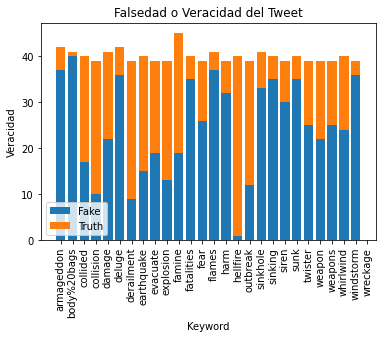
\includegraphics[width=1.0\linewidth]{keyword3}
	\caption[]{Frecuencia y \% de veracidad por keywords}
\end{figure}

\section{Más mencionados según veracidad}

Otro an\'alisis que resulta interesante es identificar a que cuentas de twitter arroban al momento de un desastre natural. Para ello extraimos usando el API de Tweepy todas las instancias que se arrobaron cuentas, y luego los graficamos. En los siguientes dos gr\'aficos podemos observar los resultados. 


 \begin{figure}[H]
	
	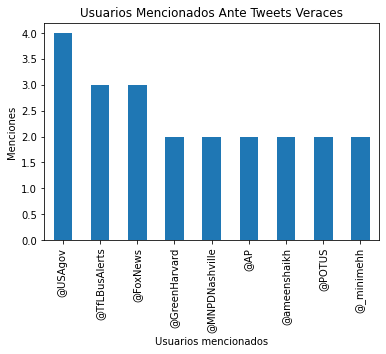
\includegraphics[width=0.70\linewidth]{arroba}
 	\caption[]{Usuarios Mencionados Ante Tweet Veraces}
\end{figure}
 \begin{figure}[H]
	
	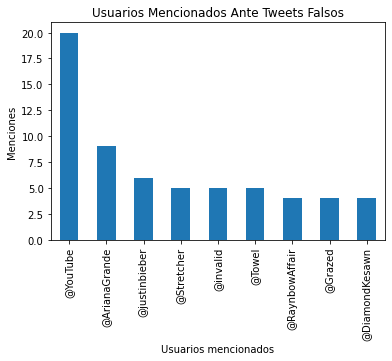
\includegraphics[width=0.70\linewidth]{arroba2}
 	\caption[]{Usuarios Mencionados Ante Tweet Falsos}
\end{figure}

Podemos observar que durante una catastrofe natural, los usuarios con m\'as menciones incluyen: distintas partes del gobierno, entre ellos el Presidente de los Estados Unides, distintos medios period\'isticos tal como Fox News y la Prensa Asociada (AP), fuerzas de seguridad, probablamente en lugares donde hayan ocurrido estos hechos ect. Todos estos usuarios son consistentes con el ejercicio. \\

A su vez, los tweets que no tienen que ver con desastres naturales, etiquetan a distintas personas que no tienen ning\'un impacto en solucionar el problema, usuarios como la p\'agina de Youtube, disintos artistas famosos tal como Justin Bieber y Ariana Grande. Estos tweets no nos permiten sacar conclusiones relevantes sobre los hechos que nos interesa.

\section{An\'alisis Heatmap}

Se utilizo un heatmap para ver la intensidad de la correlación entre la variable  de longitud del tweet contra el target. Del mismo se obtiene un valor cercano a 0,1. Lo que nos conllevaría a no incurrir en que la cantidad de caracteres utilizados permita ser un indicador sobre la veracidad del mismo.

 \begin{figure}[H]
	
	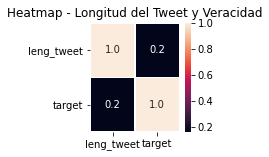
\includegraphics[width=0.70\linewidth]{heatmap}
	\caption[]{Heatmap entre Longitud del Tweet y Veracidad}
\end{figure}

\section{Conclusi\'on}

Luego de realizar an\'alisis explotaratorio de los datos, y realizar distintas visualizaciones pudimos encontrar que existen relaciones entre distintas variables. Entre ellas destamos:
\begin{itemize}
	\item La menci\'on de cuentas oficiales gubernamentales, o de medios aumentan la probabilidad de que el tweet este relacionado con cat\'astrofes naturales.
	\item Existen keywords cuyo \% de veracidad es muy alto, por lo que habr\'ia que hacer un analisis detallado para poder identificarlo. 
	\item La relaci\'on entre la longitud del tweet y la veracidad queda demostrado a nivel gr\'afico sin embargo cuando analizamos la matriz de correlaci\'on no pudimos ratificarlo. En este ejercicio ponemos m\'as peso que sacamos de la conclusi\'on visual que el m\'etodo obtenido por el m\'etodo estad\'istico. 
\end{itemize}


\end{document}
